\subsection{UC28 - Annullamento dell'ordinazione}\label{usecase:28}
\begin{figure}[H]
    \centering
    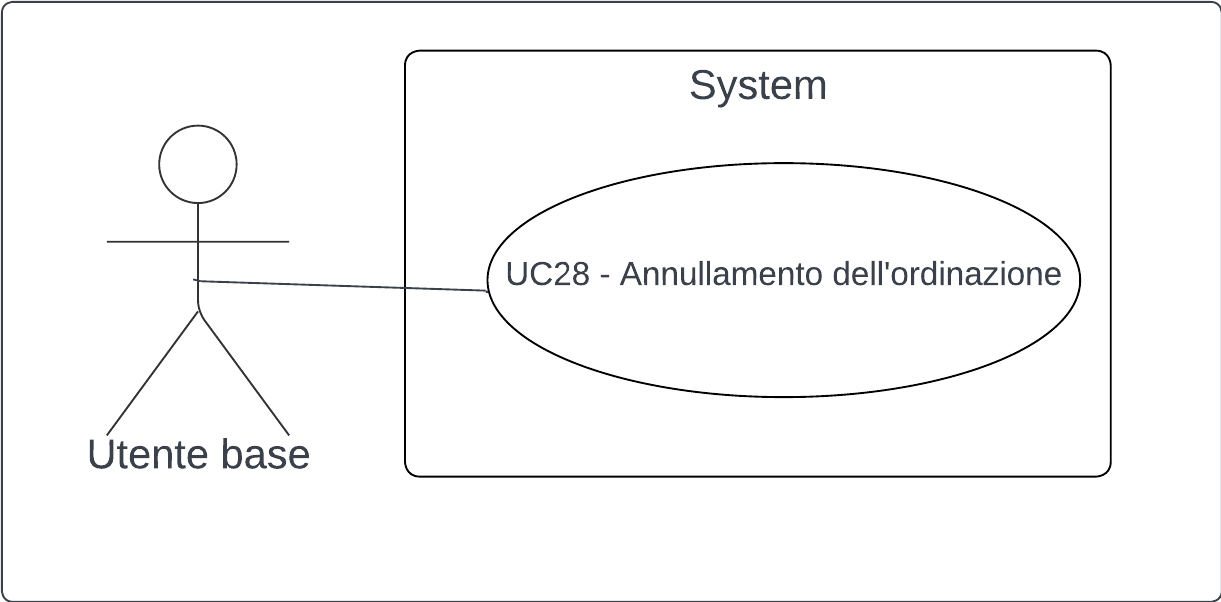
\includegraphics[width=0.9\linewidth]{ucd/UCD28.png}
\end{figure}
\textbf{Attori}:
\begin{itemize}
    \item Utente base
\end{itemize}
\textbf{Precondizioni}:
\begin{itemize}
    \item L'utente è autenticato
    \item L'utente ha creato un'ordinazione collaborativa (\nameref{usecase:3})
    \item Il tempo utile per annullare l'ordinazione non è scaduto
\end{itemize}
\textbf{Postcondizioni}:
\begin{itemize}
    \item L'utente ha annullato l'ordinazione collaborativa dei pasti e la prenotazione si trova senza ordinazioni
\end{itemize}
\textbf{\textit{Scenario}_G principale}:
\begin{enumerate}
    \item L'utente sceglie l'opzione di annullamento dell'ordinazione collaborativa
    \item Il sistema annulla l'ordinazione associate alla prenotazione e invia una notifica a tutti gli utenti associati a quella prenotazione
\end{enumerate}
\newpage